\subsection{Experimental Results}

\subsubsection{Titration curve of HCl with NaOH}
\begin{figure}[ht]
	\centering
	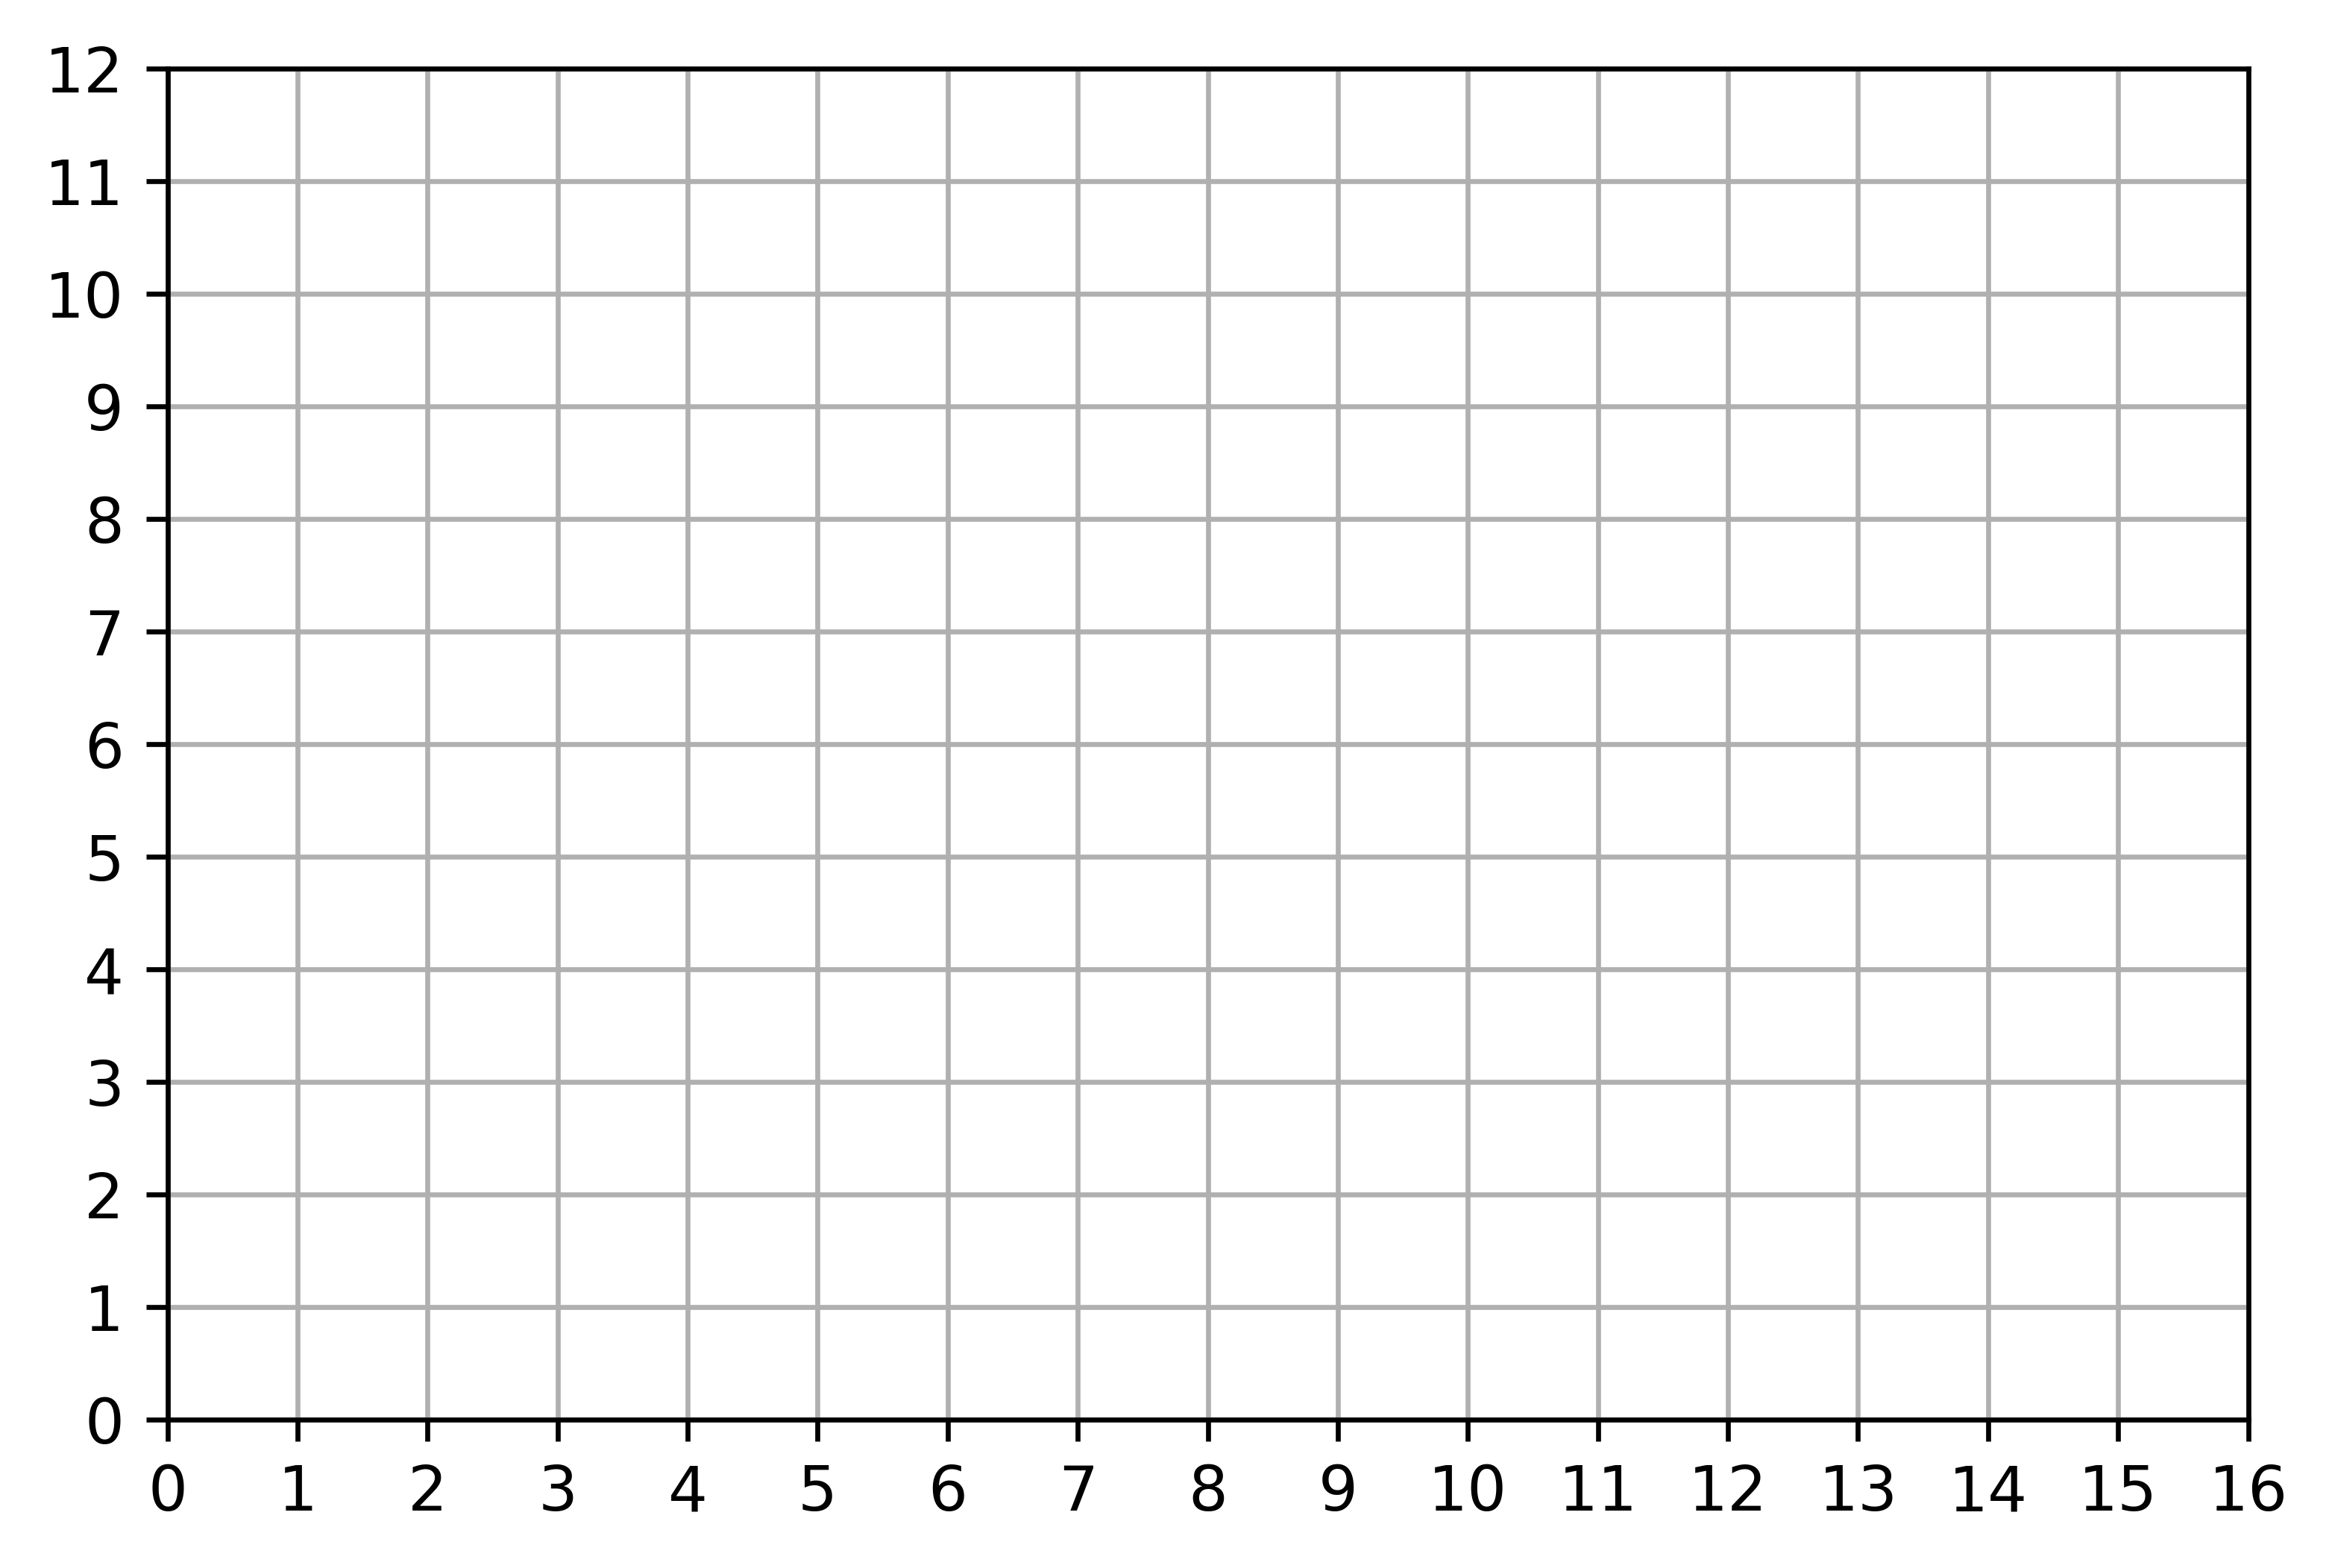
\includegraphics[width=140mm]{chem}
\end{figure}
Determine:
\begin{itemize}[label=-]
	\item pH at equivalence point:
	\item Titration jump pH:
\end{itemize}

\subsubsection{Experiment 2}
\begin{table}[ht]
	\centering
	{\renewcommand{\arraystretch}{1.75}
	\begin{tabular}{|c|p{2cm}|p{2cm}|p{2cm}|p{2cm}|p{2cm}|p{2cm}|}
		\hline
		No. & $V_{\ch{HCl}}$ ($ml$)& $V_{\ch{NaOH}}$ ($ml$) & $C_{\ch{NaOH}}$ ($N$) & $V_{\ch{HCl}}$ ($N$) & Deviation \\ \hline
		1 & & & & & \\ \hline
		2 & & & & & \\ \hline
	\end{tabular}}	
\end{table}
\vspace{-0.1cm}
\[\Delta \overline{C_{\ch{HCl}}} = \hspace{8.3cm}\] \vspace{0cm}
\[\overline{C_{\ch{HCl}}} = \hspace{8cm}\]
\newpage
\subsubsection{Experiment 3}
\begin{table}[ht]
	\centering
	{\renewcommand{\arraystretch}{1.75}
		\begin{tabular}{|c|p{2cm}|p{2cm}|p{2cm}|p{2cm}|p{2cm}|p{2cm}|}
			\hline
			No. & $V_{\ch{HCl}}$ ($ml$)& $V_{\ch{NaOH}}$ ($ml$) & $C_{\ch{NaOH}}$ ($N$) & $V_{\ch{HCl}}$ ($N$) & Deviation \\ \hline
			1 & & & & & \\ \hline
			2 & & & & & \\ \hline
	\end{tabular}}
\end{table}
\vspace{-0.1cm}
\[\Delta \overline{C_{\ch{HCl}}} = \hspace{8.3cm}\] \vspace{0cm}
\[\overline{C_{\ch{HCl}}} = \hspace{8cm}\]

\subsubsection{Experiment 4}
\begin{table}[ht]
	\centering
	{\renewcommand{\arraystretch}{1.75}
		\begin{tabular}{|c|p{3cm}|p{2.5cm}|p{2cm}|p{2cm}|p{2.5cm}|}
			\hline
			No. & Indicator & $V_{\ch{CH3COOH}}$ ($ml$) & $V_{\ch{NaOH}}$ ($ml$) & $C_{\ch{NaOH}}$ ($N$) & $C_{\ch{CH3COOH}}$ ($N$)\\ \hline
			1 & Phenolphthalein & & & & \\ \hline
			2 & Methyl orange & & & & \\ \hline
	\end{tabular}}
\end{table}

\subsection{Answer the questions}
\begin{enumerate}
	\item When changing the concentration of HCl or NaOH, does the titration curve changes accordingly? Explain.
	
	The titration curve will not change since the chemical equivalence of reactants stays the same. Only titration jump varies according to the concentration:\\
	- Decrease in concentration results in a short titration jump.\\
	- Increase in concentration results in a long titration jump.
	
	\item If we were to find the concentration of HCl, determine from experiments 2 and 3 the experiment yielding higher accuracy.
	
	Phenolphthalein contributes to accurate result since the titration jump of the indicator is ranging from 8 to 10. However, the jump of metyl orange varies from 3.1 to 4.4, which is further from the equivalence point than that of phenolphthalein. Therefore, experiment 2 using phenolphthalein yields high accuracy.
	
	\item From the result of experiment 4, which indicator is more accurate when determining the concentration of \ch{CH3COOH} solution?
	
	Phenolphthalein gives more accurate result than methyl orange. In acidic environment, phenolphthalein has an advantage of being transparent and only visible in basic solution through its distinctive violet color. In contrast, the change in color of methyl orange is much harder to observe (red in acidic environment to orange-yellow in basic environment).
	
	\item In volumetric titration, if NaOH and HCl were interchanged, would the result be changed accordingly? Explain.
	
	The result remained consistent since the initial properties of the reaction stays the same (it is a neutralization reaction and will change the color of an indicator at equivalence point).
\end{enumerate}